% This file is part of CrashOS and is released under GPLv2 (see crashos/LICENSE.md)
% Copyright Airbus Group

%\documentclass[a4paper,11pt]{article}
\documentclass[12pt, openany]{report}
%\documentclass{report}

%\usepackage[ps2pdf,bookmarks=true,bookmarksnumbered=true]{hyperref}
\usepackage[utf8x]{inputenc}
\usepackage[T1]{fontenc}
\usepackage[french]{babel}
\usepackage{lmodern}
\usepackage[dvips]{graphicx}
\usepackage{xcolor}
\usepackage{float}
\usepackage{hyperref}
\usepackage{array}
\usepackage{multirow}
\usepackage{longtable}


\usepackage{listings}
\definecolor{codegreen}{rgb}{0,0.5,0}
\definecolor{codegray}{rgb}{0.5,0.5,0.5}
\definecolor{codepurple}{rgb}{0,0,0.82}
\definecolor{codeplop}{rgb}{0.5,0,0.82}
\definecolor{backcolour}{rgb}{0.92,0.92,0.92}
\lstdefinestyle{mystyle}{
    backgroundcolor=\color{backcolour},   
    commentstyle=\color{codegreen},
    keywordstyle=\color{codeplop},
    numberstyle=\tiny\color{codegray},
    stringstyle=\color{codepurple},
    basicstyle=\footnotesize,
    breakatwhitespace=false,         
    breaklines=true,                 
    captionpos=b,                    
    keepspaces=true,                 
    numbers=left,                    
    numbersep=5pt,                  
    showspaces=false,                
    showstringspaces=false,
    showtabs=false,                  
    tabsize=2
}
\lstset{style=mystyle}
%\usepackage{tabularx}
%\usepackage{array}
%\usepackage{alltt}
%\usepackage{rotating}
%\usepackage{fancyhdr}
%\usepackage{fancybox}

\newcommand{\tech}[1]{{\footnotesize\texttt{#1}}}

% \setlength{\parindent}{0mm}
% \setlength{\parskip}{4mm}

\begin{document}

\title{CrashOS documentation}
\author{Anaïs Gantet}
\date{March-September 2016}
\maketitle
\tableofcontents

%%%%%%%%%%%%%%%%%%%%%%%%%%%%%%%%%%%%%%%%%%%%%%%%%%%%%%%%%%%%%%%%%%%%%%%%%%%%%%%%%%%%%%%%%%%%%%%%%%%%%%%%%%%%%%%%%%%%%%%%%%%
\newpage
\section*{What is CrashOS?}
\addcontentsline{toc}{section}{What is CrashOS?}
\paragraph{}CrashOS is a tool dedicated to the research of vulnerabilities in hypervisors by creating unusual system configurations. 
\paragraph{}CrashOS is a minimalist Operating System, containing the kernel as well as a list of tests which aim to lead to hypervisor crashs, hence its name. You can launch existing tests or implement your owns and observe hypervisor behaviour towards this unusual kernel.

\paragraph{}The core of CrashOS provides the following OS features: 
\begin{itemize}
	\item The Boot entry
	\item The memory management (segmentation and paging)
	\item The interrupt and exception handling
	\item The I/O communication
\end{itemize}
A default kernel configuration is available but this set of features allows to entirely reconfigure the kernel as you desire.

%%%%%%%%%%%%%%%%%%%%%%%%%%%%%%%%%%%%%%%%%%%%%%%%%%%%%%%%%%%%%%%%%%%%%%%%%%%%%%%%%%%%%%%%%%%%%%%%%%%%%%%%%%%%%%%%%%%%%%%%%%%
\section*{Hardware and software requirements}
\addcontentsline{toc}{section}{Hardware and software requirements}

\paragraph{}CrashOS only works on Intel x86 hardware architecture and requires gcc-4.8 to be compiled and GRUB to boot.

%%%%%%%%%%%%%%%%%%%%%%%%%%%%%%%%%%%%%%%%%%%%%%%%%%%%%%%%%%%%%%%%%%%%%%%%%%%%%%%%%%%%%%%%%%%%%%%%%%%%%%%%%%%%%%%%%%%%%%%%%%%
\section*{CrashOS installation}
\addcontentsline{toc}{section}{CrashOS installation}

\paragraph{}To install CrashOS, first compile the project with the main Makefile. It will create the 32-bits executable file \emph{test.bin}. 
\begin{lstlisting}
.../crashos$ make
\end{lstlisting}
Then install \emph{test.bin} and Grub in a bootable storage, and use this bootable storage to launch the VM in your hypervisor.
\\A example of installation with Vmware is included in the Makefile by executing the following command line:
\begin{lstlisting}
.../crashos$ make install
\end{lstlisting}
Don't forget to adapt the VM path in the script \emph{/tools/installer\_vmware.sh}:
\begin{lstlisting}
VMPATH="/home/anais/Vmware/${VMNAME}"
\end{lstlisting}

%%%%%%%%%%%%%%%%%%%%%%%%%%%%%%%%%%%%%%%%%%%%%%%%%%%%%%%%%%%%%%%%%%%%%%%%%%%%%%%%%%%%%%%%%%%%%%%%%%%%%%%%%%%%%%%%%%%%%%%%%%%
\section*{CrashOS binary structure}
\addcontentsline{toc}{section}{CrashOS binary structure}
\paragraph{}The CrashOS binary structure is defined by the linker \emph{/build/linker.lds}.
\paragraph{}CrashOS is compatible with the multiboot format to be loaded by Grub. Its entry point is located at 0x200000. The CrashOS binary file contains several sections: \emph{.text} contains the kernel core, \emph{.tests\_init}, \emph{.tests} and \emph{.tests\_restore} the test list, and \emph{.real\_mode} the real mode code if needed.
%%%%%%%%%%%%%%%%%%%%%%%%%%%%%%%%%%%%%%%%%%%%%%%%%%%%%%%%%%%%%%%%%%%%%%%%%%%%%%%%%%%%%%%%%%%%%%%%%%%%%%%%%%%%%%%%%%%%%%%%%%%
\section*{CrashOS core organisation}
\addcontentsline{toc}{section}{CrashOS core organisation}
The CrashOS core is divided in two parts:
\begin{itemize}
	\item The kernel part: it contains all OS functions regarding the memory management, the interrupt handling and the I/O communication
	\item The testing part: it contains all functions regarding the test launch, the test declaration and the logs.
\end{itemize}
The figure \ref{orga} illustrates the organisation of the CrashOS core files.
\begin{figure}[H]
	\centering
	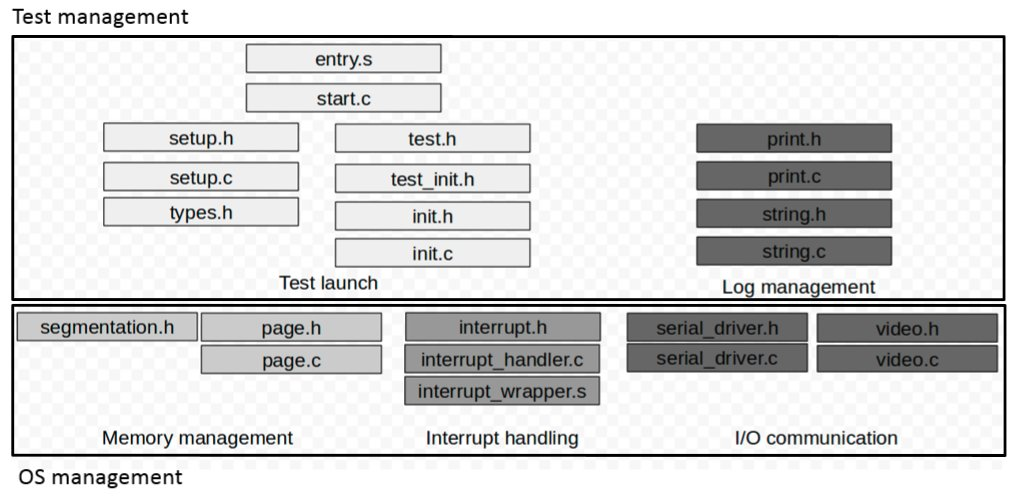
\includegraphics[width=14cm]{images/img31.jpg}
	\caption{CrashOS core files}
	\label{orga}
\end{figure}

%%%%%%%%%%%%%%%%%%%%%%%%%%%%%%%%%%%%%%%%%%%%%%%%%%%%%%%%%%%%%%%%%%%%%%%%%%%%%%%%%%%%%%%%%%%%%%%%%%%%%%%%%%%%%%%%%%%%%%%%%%%
\section*{CrashOS: How does it work?}
\addcontentsline{toc}{section}{CrashOS: How does it work?}

\subsection*{CrashOS start}

\paragraph{} CrashOS is loaded by Grub at 0x200000. The entry point of CrashOS, contained in \emph{/src/core/entry.s}, initializes the stack pointer and calls the start function. 
\begin{lstlisting}[language=c]
entry:
        cli
        movl    $__kernel_start__, %esp
        pushl   $0
        popf
        movl    %ebx, %eax
        call    start
\end{lstlisting}
The start function, implemented in \emph{/src/core/start.c}, essentially handle the launch of all tests listed in the \emph{.tests} section. At this stage, the kernel is not configured yet. The kernel configuration is proper to each test and must be implemented by the test.
\subsection*{Fill the .tests section}
The macro DECLARE\_TEST has been defined in \emph{/src/core/test.h}:
\begin{lstlisting}[language=c]
typedef int (*test_t)(); 
#define DECLARE_TEST(xXx)   test_t * __attribute__((section(".tests"))) xXx##_ptr = &xXx;
\end{lstlisting}
To declare a function as a test and store it in the \emph{.tests} section, just use this macro as following:
\begin{lstlisting}[language=c]
DECLARE_TEST(mytest)
\end{lstlisting}

\subsection*{CrashOS test format}

\paragraph{}In CrashOS, each test needs to define a specific kernel configuration. Thus, each test must contain:
\begin{itemize}
	\item An "init" function: it saves the current kernel configuration and defines the configuration with which we want to work
	\item The "test" function
	\item A "restore" function: it recovers the old kernel configuration
\end{itemize}
A test template is available in \emph{/templates/test\_template.txt}.


%%%%%%%%%%%%%%%%%%%%%%%%%%%%%%%%%%%%%%%%%%%%%%%%%%%%%%%%%%%%%%%%%%%%%%%%%%%%%%%%%%%%%%%%%%%%%%%%%%%%%%%%%%%%%%%%%%%%%%%%%%%
\section*{CrashOS usage}
\addcontentsline{toc}{section}{CrashOS: some uses}

\paragraph{} Specify, in the main Makefile, the list of tests you want to launch
	\begin{lstlisting}[caption=CrashOS Makefile: example of test list]
	...
	TESTS :=  tests_REP_OUTS/test_01 tests_REP_OUTS/test_02 
	...
	\end{lstlisting}

\subsection*{Launch existing tests}


\paragraph{}CrashOS provides some examples of tests described below:

\setlongtables
\begin{longtable}{|l | l |}
\hline
test\_01 & "REP OUTS COM3" instruction using a DS mapped on non \\
         & consecutive physical pages\\
\hline
test\_02 & "REP OUTS COM3" instruction using a DS\_r3 mapped on \\
         & non consecutive physical pages and a pb in virtual pages\\
         & access rights\\
\hline
test\_03 & "REP OUTS COM1" instruction using a DS mapped on non \\
         & consecutive physical pages (with 0x67 prefix)\\
\hline
test\_04 & "REP OUTS COM1" instruction using a DS mapped on non \\
         & consecutive physical pages + Reading out of the segment limit\\
\hline
test\_05 & Writing more than 0x82 (=130) bytes into serial port COM1\\
\hline
test\_06 & Launch all privileged instructions in ring 3. Must cause a GP\\
\hline
test\_07 & "REP INS/OUTS COM1 ring 3" instruction is using a DS\_r3 \\
         & mapped on non consecutive physical pages and a pb in virtual\\
         & pages access rights\\
\hline
test\_08 & "REP OUTS COM1" instruction performed in ring 3 which uses\\
        & data of a kernel page\\
\hline
test\_09 & Launch all sensitive un-privileged instructions in ring 3 \\
         & with a bad paging configuration (kernel page)\\
\hline
test\_10 & Try to execute sensible instructions placing between 2 pages\\
\hline
test\_11 & VMXON tests with a bad configuration (CR4.VMXE, MSR:0x3a,...)\\
         & to verify if exceptions occur as expected\\
\hline
test\_12 & VMXON tests with a bad configuration (CR4.VMXE, MSR:0x3a,...)\\
         & to verify if exceptions occur as expected\\
\hline
test\_13 & first REP OUTS fuzzer \\
&- privilege level : ring 0 \\
&- instruction     : REP OUTS \\
&- port range      : [0x00000000 - 0xffffffff] (non sense : io port size : 16 bits)\\
&- buffer addr     : 0x300000 (no paging)\\
&- buffer size     : 1\\
&- buffer content  : 'A'\\
\hline
test\_14 &  REP OUTS fuzzer - understanding Ramooflax and port 0x92\\
&- privilege level : ring 0\\
&- instruction     : REP OUTS\\
&- port range      : 0x****0092\\
&- buffer addr     : 0x300000 (no paging)\\
&- buffer size     : 1\\
&- buffer content  : 'A'\\
\hline
test\_15 & REP OUTS fuzzer - list of fails - value 'B' and 'A'\\
&- privilege level : ring 0\\
&- instruction     : REP OUTS\\
&- port range      : [0x0000 - 0xffff]\\
&- buffer addr     : 0x300000 (no paging)\\
&- buffer size     : 1\\
&- buffer content  : 'B' and 'A'\\
\hline
test\_16 & REP OUTS fuzzer - understanding critical io ports\\
&- privilege level : ring 0\\
&- instruction     : REP OUTS\\
&- port number     : 0x92, 0x102c, 0x1042, 0x2000, 0xcf9\\
&- buffer addr     : 0x300000 (no paging)\\
&- buffer size     : 1\\
&- buffer content  : range [0x00-0xff]\\
\hline
test\_17 & REP OUTS fuzzer - test buffer address\\
&- privilege level : ring 0\\
&- instruction     : REP OUTS\\
&- port number     : 0x3f8\\
&- buffer addr     : [0x00000000-0xffffffff] (no paging)\\
&- buffer size     : 1\\
&- buffer content  : the real memory \\
\hline
test\_18 & REP OUTS fuzzer - all values/ports in RING 0 \\
&- privilege level : ring 0\\
&- instruction     : REP OUTS\\
&- port number     : [0x0000-0xffff]\\
&- buffer addr     : 0x300000 (no paging)\\
&- buffer size     : 1\\
&- buffer content  : range [0x00-0xff]\\
\hline

\end{longtable}

You can use this test base to begin to test your hypervisor.



\subsection*{Develop your own test}
You can also develop your own test. 
\\Use the script \emph{/tools/create\_new\_test\_directory.py} to create a new directory containing your test. It will create the local Makefile, a log file to store the test logs, a text file to describe the test and the test file filled with the test template.
\begin{lstlisting}
/crashos/tools$ python create_new_test_directory.py myowntest
Directory myowntest created
/crashos/tools$ cd ..
/crashos$ ls src/myowntest/
Makefile  myowntest.c  myowntest.log  myowntest.txt
\end{lstlisting}

\paragraph{Init functions}To init the kernel, some default functions are available in src/core/init.h and src/core/init.c.

\setlongtables
\begin{longtable}{|l | l |}
\hline
init\_work\_mem() 		& Initialize the mem\_info struct to define the available \\
						& physical memory\\
\hline
init\_segmentation(...)	& Initialize the GDT (Global Descriptor Table) with the \\
						& following entries and update gdtr and segment selectors\\
\hline
init\_paging(...) 		& Initialize the PGD with the first 4MB in Identity Mapping, \\
						& update CR3 and CR4 and enable the paging in CR0 \\
\hline
init\_interrupts(...) 	& Initialize the IDT (Interrupt Descriptor Table) with the\\ 
						& following entries (32 first entries for exceptions)\\
 \hline
\end{longtable}


\paragraph{Other functions}Others functions allow the developer to modify the default system parameters and to define his own configuration. The following command line generates a a code documentation for all functions available in CrashOS :
\begin{lstlisting}
.../crashos$ make doc
\end{lstlisting}
It creates a html documentation in doxygen\_documentation/html/index.html.
\end{document}
